\section{Results}
\label{sec:results}

%%%%%%%%%%%%%% usage behavior
%\item We characterize \textbf{usage behaviors} and show that aggregate network usage seen by the ISP does not show a trough in the middle of the day for high capacity tiers.
%, as observed by aggregate usage across all tiers. % This motivates the need to study usage per tier separately as usage behavior differs with tiers.
%%%%%%%%%%%%%% prime time
%\item We reaffirm the importance of measuring performance during the prime-time peak hours, and urge the FCC to revisit and standardize the measurement and interpretation of \textbf{prime-time ratio}. 
%we show through our analysis that the \textbf{prime-time ratio
%(ratio of average data rate during prime time hours to non prime time hours)
%does not follow the conventional definition stated by the FCC.
%%%%%%%%%%%%% different perspective of utilization
%\item We shed light on the user's and ISP's \textbf{differing perspectives of \emph{capacity utilization}}, and show that indeed, the user's behavior does change when offered a higher capacity link even though the overall utilization stops increasing after a certain upper limit.
%%%%%%%%%%%%% user taxonomy and multiple benchmarks
%\item We suggest that the FCC adopt multiple benchmarks to better characterize broadband availability, deployment, and adoption in the US, based on our analysis of varying usage patterns within the same ISP tier.
%We explore a taxonomy of different users based on varying traffic patterns of users within the same capacity tier, and 

\todo{This is the results section}

We present a comparison between the usage characteristics of the control\footnote{gateway byte counters from users with a 105 Mbps access link} and test\footnote{gateway byte counters from users with a 105 Mbps access link}. We interpret the results as change in usage behavior due to increase in access link bandwidth. %although these are two separate sets of devices we interpret them as changes as explained in "methodology" or "data"

%------------------------------------------------------------------------------

\subsection{User Behavior}
\label{subsec:behavior}

\hypoth{1}. Does aggregate user behavior differ?


\begin{itemize}
\itemsep0em 
\item Figure ~\ref{fig:TS-data-rate-daily}
\item Plot the aggregate data rate using bytes transferred per 15 min slot. 
\item Average across devices, then aggregate across days for each time slot.
\item Peak data rates are reached between 8PM-12AM (2-6 UTC) \todo{replace with fixed time plot}.
\item Usual average usage patterns have a small peak in the morning (10AM), then dip, and then rise up again in the evening ~\cite{sandvine2014report1}. In contrast, there is no trough in the average usage for the patterns observed in our set.
\item No troughs is consistent even on patterns observed weekly instead of daily.
\end{itemize}


%%%%%%%%%%%%%%%%%%%%%%%%%%%%%%%%%%%%%%%%%%%%%%%%%%%%%%%%%%%%%%%%%%%%%
\begin{figure}[ht!]
%\hspace*{-0.2in}
\begin{minipage}{\linewidth}
\centering
%
%\hfill
\begin{subfigure}[b]{\linewidth}
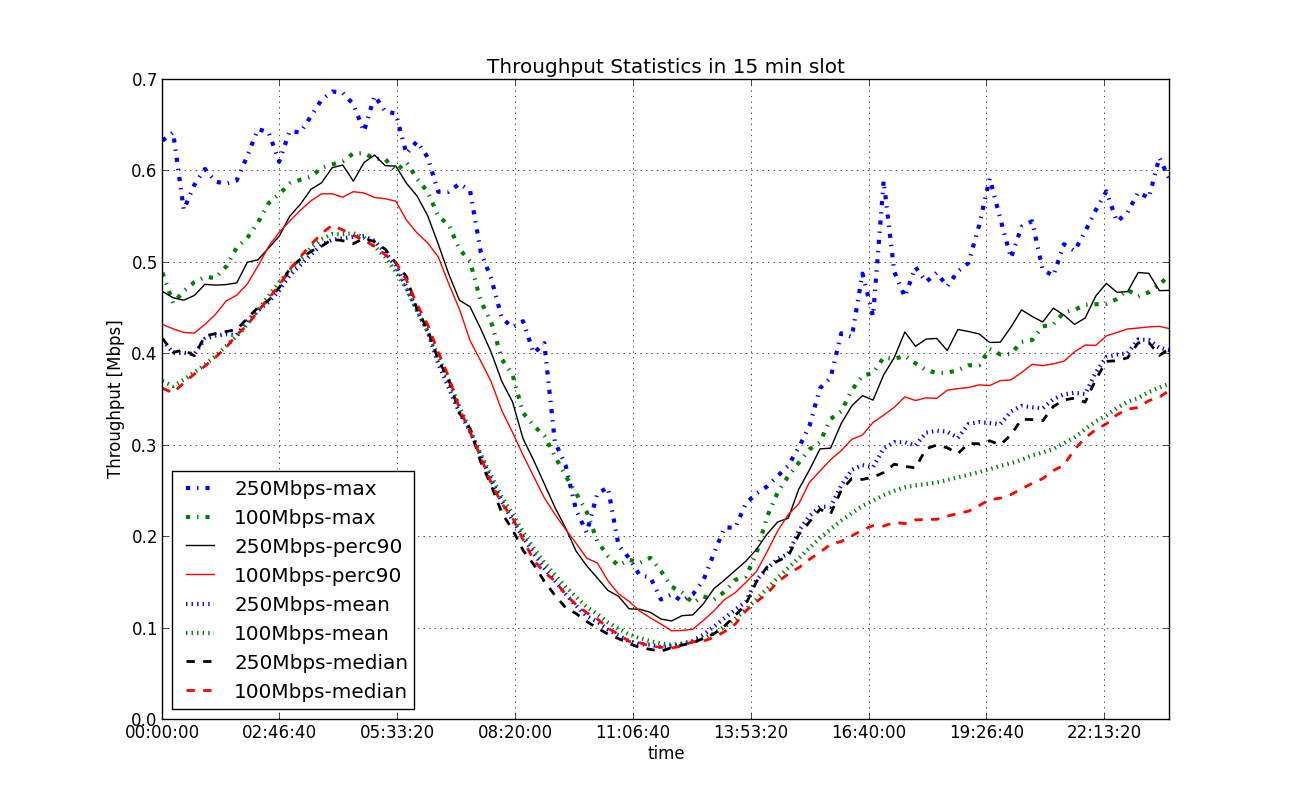
\includegraphics[width=\linewidth]{figures/describe-total-throughput-per-day[replace].png}
  \caption{agg (days) over means (devices)}
  %http://riverside.noise.gatech.edu:8083/separated/full/describe-total-throughput-per-day.png
  \label{fig:TS-data-rate-daily}
\end{subfigure}
%
\vspace{-1em}
%
\begin{subfigure}[b]{0.90\linewidth}
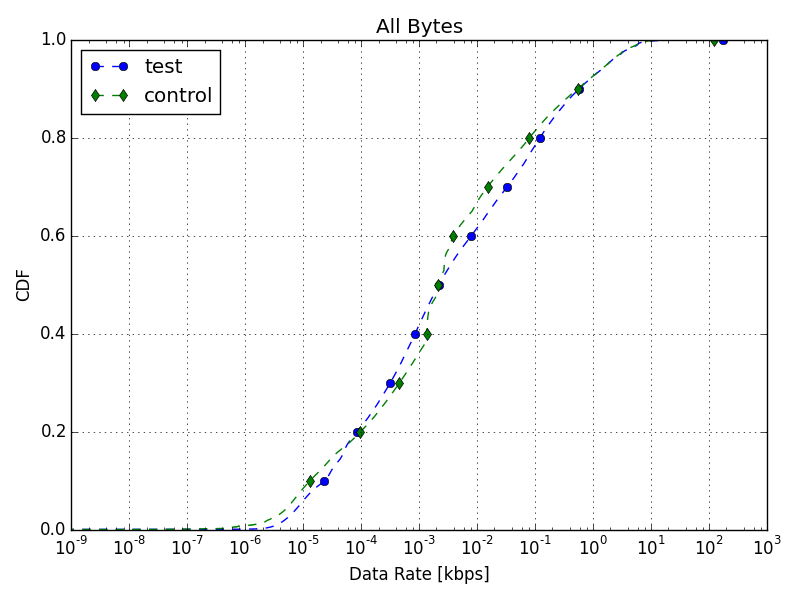
\includegraphics[width=\linewidth]{figures/cdf-all-bytes.png}
  \caption{CDF of data rate per time slot for all devices (agg view of data)}
  \vspace{1em}
  %http://sites.noise.gatech.edu/~sarthak/files/comcast/plots/full_dw/cdf-all-bytes.png
  \label{fig:CDF-data-rate-all}
\end{subfigure}
%\hfill
\end{minipage}
\caption{User Behavior: Overall not much change due to capacity increase}
\label{fig:user-behavior}
% created using docs/metadata-separated.log
\end{figure}
%%%%%%%%%%%%%%%%%%%%%%%%%%%%%%%%%%%%%%%%%%%%%%%%%%%%%%%%%%%%%%%%%%%%%


\begin{itemize}
\itemsep0em 
\item Figure ~\ref{fig:CDF-data-rate-all}
\item Distribution of average data rate (kbps) per 15-min time slot 
\item Very similar distributions of bytes transferred
\item Median data rate ~ 2bps for 3 months x thousands of devices!
\end{itemize}


%------------------------------------------------------------------------------

\subsection{Peak Utilization}
\label{subsec:peak-util}

\hypoth{2}. Does the maximum (or 90-\%ile) data transferred by the device differ?

\begin{itemize}
\itemsep0em 
\item Figure ~\ref{fig:CDF-data-rate-max}
\item Calculate the maximum data rate for a device over the three months, and compare max rate (per device) for test set and max rate (per device) for control set
\item test set has higher (max) average data rate below 10 kbps \todo{sanity check numbers, redo plot}
\item 30\% of devices in the control set have a max data rate of 2 kbps while 30\% of test set has a max data rate of 10 kbps.
\end{itemize}

%%%%%%%%%%%%%%%%%%%%%%%%%%%%%%%%%%%%%%%%%%%%%%%%%%%%%%%%%%%%%%%%%%%%%
\begin{figure}[ht!]
%\hspace*{-0.2in}
\begin{minipage}{0.90\linewidth}
\centering
%
%\hfill
\begin{subfigure}[b]{0.90\linewidth}
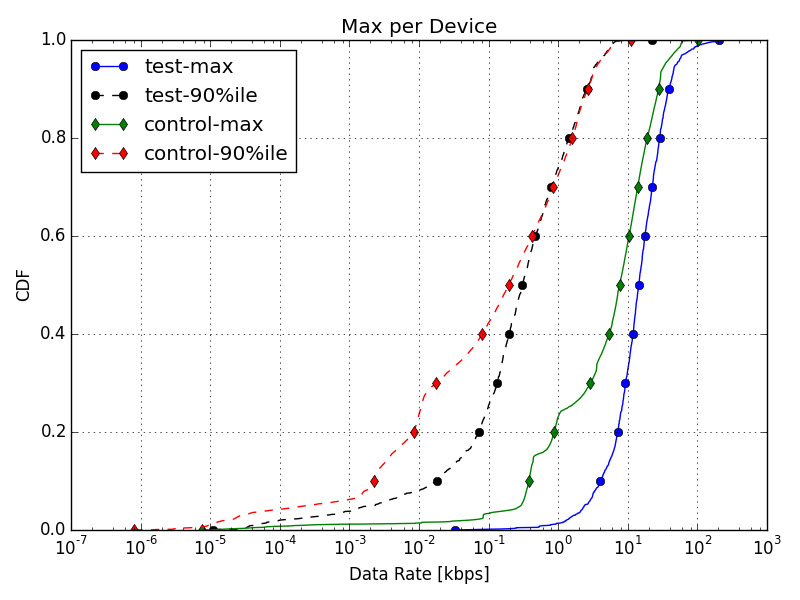
\includegraphics[width=\linewidth]{figures/cdf-max-per-device.png}
  \caption{CDF of max per device}
  %http://sites.noise.gatech.edu/~sarthak/files/comcast/plots/full_dw/cdf-max-per-device.png
  \label{fig:CDF-data-rate-max}
\end{subfigure}
%
\vspace{-1em}
%
\begin{subfigure}[b]{0.90\linewidth}
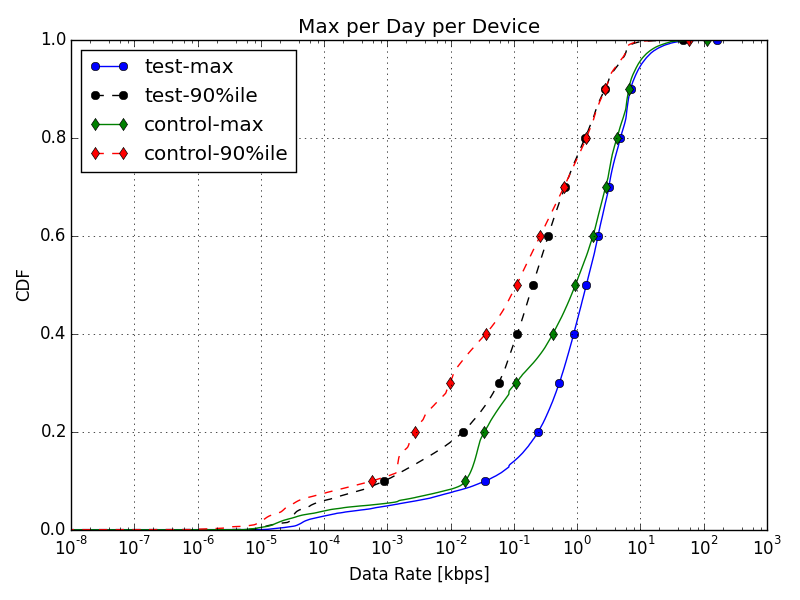
\includegraphics[width=\linewidth]{figures/cdf-max-per-day-per-device.png}
  \caption{CDF of max per device daily}
  \vspace{1em}
  %http://sites.noise.gatech.edu/~sarthak/files/comcast/plots/full_dw/cdf-max-per-day-per-device.png
  \label{fig:CDF-data-rate-max-daily}
\end{subfigure}
%\hfill
\end{minipage}
\caption{Peak Utilization: The maximum data rate varies for test and control set for low data rates, and this variation is present daily.}
\label{fig:peak-utilization}
% created using docs/metadata-separated.log
\end{figure}
%%%%%%%%%%%%%%%%%%%%%%%%%%%%%%%%%%%%%%%%%%%%%%%%%%%%%%%%%%%%%%%%%%%%%

\begin{itemize}
\itemsep0em 
\item Figure ~\ref{fig:CDF-data-rate-max-daily}
\item Max seen by a device per day, in 3 months
\item Consistent increase for daily max data rate per device
\item 15 min granularity misses information
	\begin{itemize}
	\itemsep0em
	\item short faster data bursts
	\item better video quality
	\item baseline is different
	\end{itemize}
\end{itemize}


%------------------------------------------------------------------------------

\subsection{Prime Time Ratio}
\label{subsec:prime-time}

\hypoth{3}. Does the prime-time ratio differ?

\begin{itemize}
\itemsep0em 
\item Figure ~\ref{fig:TS-prime-time-ratio}
\item 8p - 12a shows a higher prime-time ratio than 7p - 11p (as stated by FCC) in the Comcast data set. The curve in convex, i.e. there is only one peak time in a day.
\item Distribution of prime time ratios over control and test set is very similar
\item The average prime-time ratio for control sets is consistently higher than test set
\item Test set has 10\% lower PT than control set
\item Diurnal pattern shows high ratio for 5 weekdays, and low ratio on weekends.
\item Also easy to see Thanksgiving, black friday, Christmas, etc. holidays
\end{itemize}



%\sg{can also include PT table from ppt if worth it -- table shows the "no dip" pattern similar to time series in first subsection.}


%%%%%%%%%%%%%%%%%%%%%%%%%%%%%%%%%%%%%%%%%%%%%%%%%%%%%%%%%%%%%%%%%%%%%

\begin{figure}[ht!]
\begin{minipage}{\linewidth}
\centering
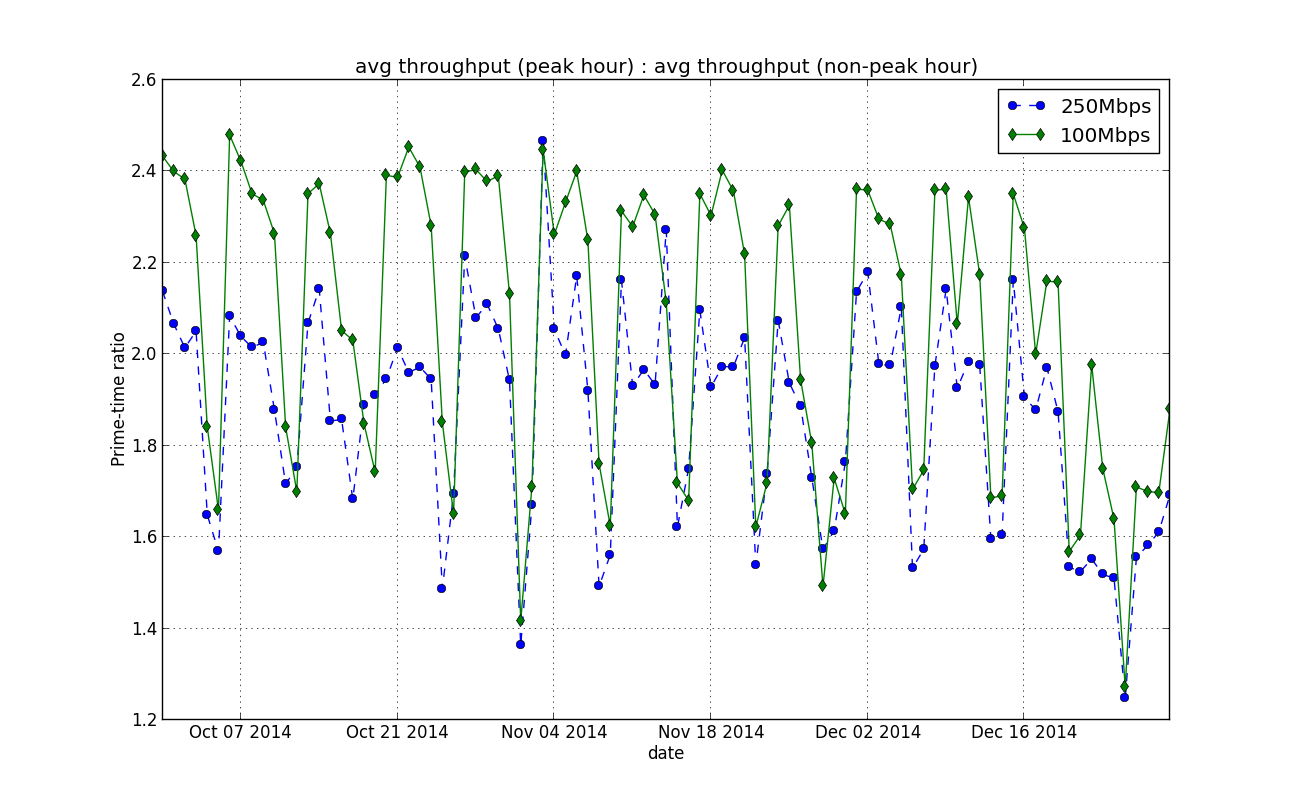
\includegraphics[width=\linewidth]{figures/prime-time-ratio-by-date[replace].png}
\caption{Prime Time ratio showing weekly pattern + differences during holiday periods (Thanksgiving, Christmas)}
%http://riverside.noise.gatech.edu:8083/separated/full/prime-time-ratio-by-date.png
\label{fig:TS-prime-time-ratio}
\end{minipage}
\end{figure}

%%%%%%%%%%%%%%%%%%%%%%%%%%%%%%%%%%%%%%%%%%%%%%%%%%%%%%%%%%%%%%%%%%%%%



% \sg{ http://riverside.noise.gatech.edu:8083/separated/full/cdf-prime-time-ratio-per-device.png not needed ? }



\begin{itemize}
\itemsep0em 
\item Figure ~\ref{fig:TS-prime-time-ratio}
\item 8p - 12a shows a higher prime-time ratio than 7p - 11p (as stated by FCC) in the Comcast data set. The curve in convex, i.e. there is only one peak time in a day.
\item Distribution of prime time ratios over control and test set is very similar
\item The average prime-time ratio for control sets is consistently higher than test set
\item Test set has 10\% lower PT than control set
\item Diurnal pattern shows high ratio for 5 weekdays, and low ratio on weekends.
\item Also easy to see Thanksgiving, black friday, Christmas, etc. holidays
\end{itemize}


%------------------------------------------------------------------------------


\subsection{Peak Ratio}
\label{subsec:peak-ratio}

\hypoth{4}. How much does the traffic vary in a single day?

\begin{itemize}
\itemsep0em 
\item Figure ~\ref{fig:CDF-peak-ratio-median}
\item test-set sees higher variance in usage per device
\item implies that ISPs should condition their networks to 50 times median usage per user
\end{itemize}


%%%%%%%%%%%%%%%%%%%%%%%%%%%%%%%%%%%%%%%%%%%%%%%%%%%%%%%%%%%%%%%%%%%%%

\begin{figure}[ht!]
\begin{minipage}{0.90\linewidth}
\centering
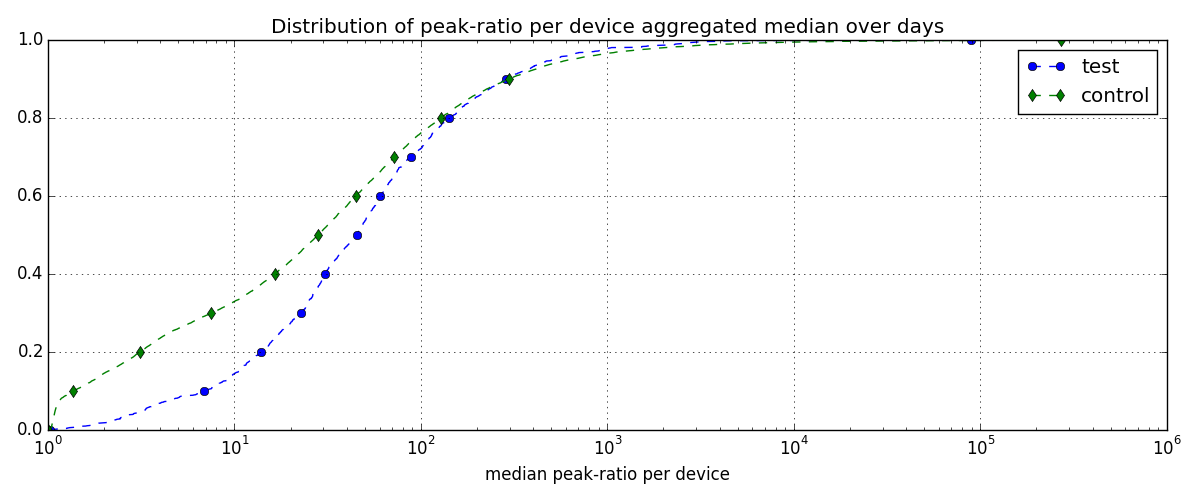
\includegraphics[width=1\linewidth]{figures/peakratio-CDF-devices-MEDIAN.png}
\caption{Median peak ratio per device showing that test set has higher daily variance, which goes upto 50 times)}
%http://sites.noise.gatech.edu/~sarthak/files/comcast/plots/full_dw/peakratio-CDF-devices-MEDIAN.png
\label{fig:CDF-peak-ratio-median}
\end{minipage}
\end{figure}



%%%%%%%%%%%%%%%%%%%%%%%%%%%%%%%%%%%%%%%%%%%%%%%%%%%%%%%%%%%%%%%%%%%%%



%
%big difference (2 x median ratio) in per device per day ratios of 90%ile:median.
%weird shape again for values < ratio 100
%big difference in this ratio per day, and it is consistent across all individual sets + months.
%very large for Dec, slightly smaller for Nov
%interestingly, at higher ratios control is slightly > test. This means that certain devices in control set have a huge std (ratio) in a day as compared to test set which has a lower “max” ratio.
%


%------------------------------------------------------------------------------


\subsection{Traffic Asymmetry}
\label{subsec:asymmetry}

\begin{itemize}
\itemsep0em 
\item \todo{maybe this doesn't need a separate section, just comment on asymmetry in each of the above}
\item Cisco vs Alcatel: upload is increasing vs there's still too much download
\item Claim that its reducing due to uploads, but content is mostly download. Is the ratio still 10:1 (FCC thinks its ~25:3)
\item Compare with Sandvine asymmetry stats
\item Talk about 3 Mbps comparison with observed uplink in control and test set
\end{itemize}



